\problemname{Jinxed Jewelry}

Eitri -- the king of the dwarfs -- is one of the mightiest blacksmiths in the universe.
And still he was paralyzed by fear when he was tasked to repair the necklace of Harmonia which broke into $n$ pieces.
It was a wonderful jewelry, but it was also as dangerous as it looked beautiful since the necklace was jinxed and brought great misfortune to who ever owned it.

\begin{figure}[h]
	\centering
	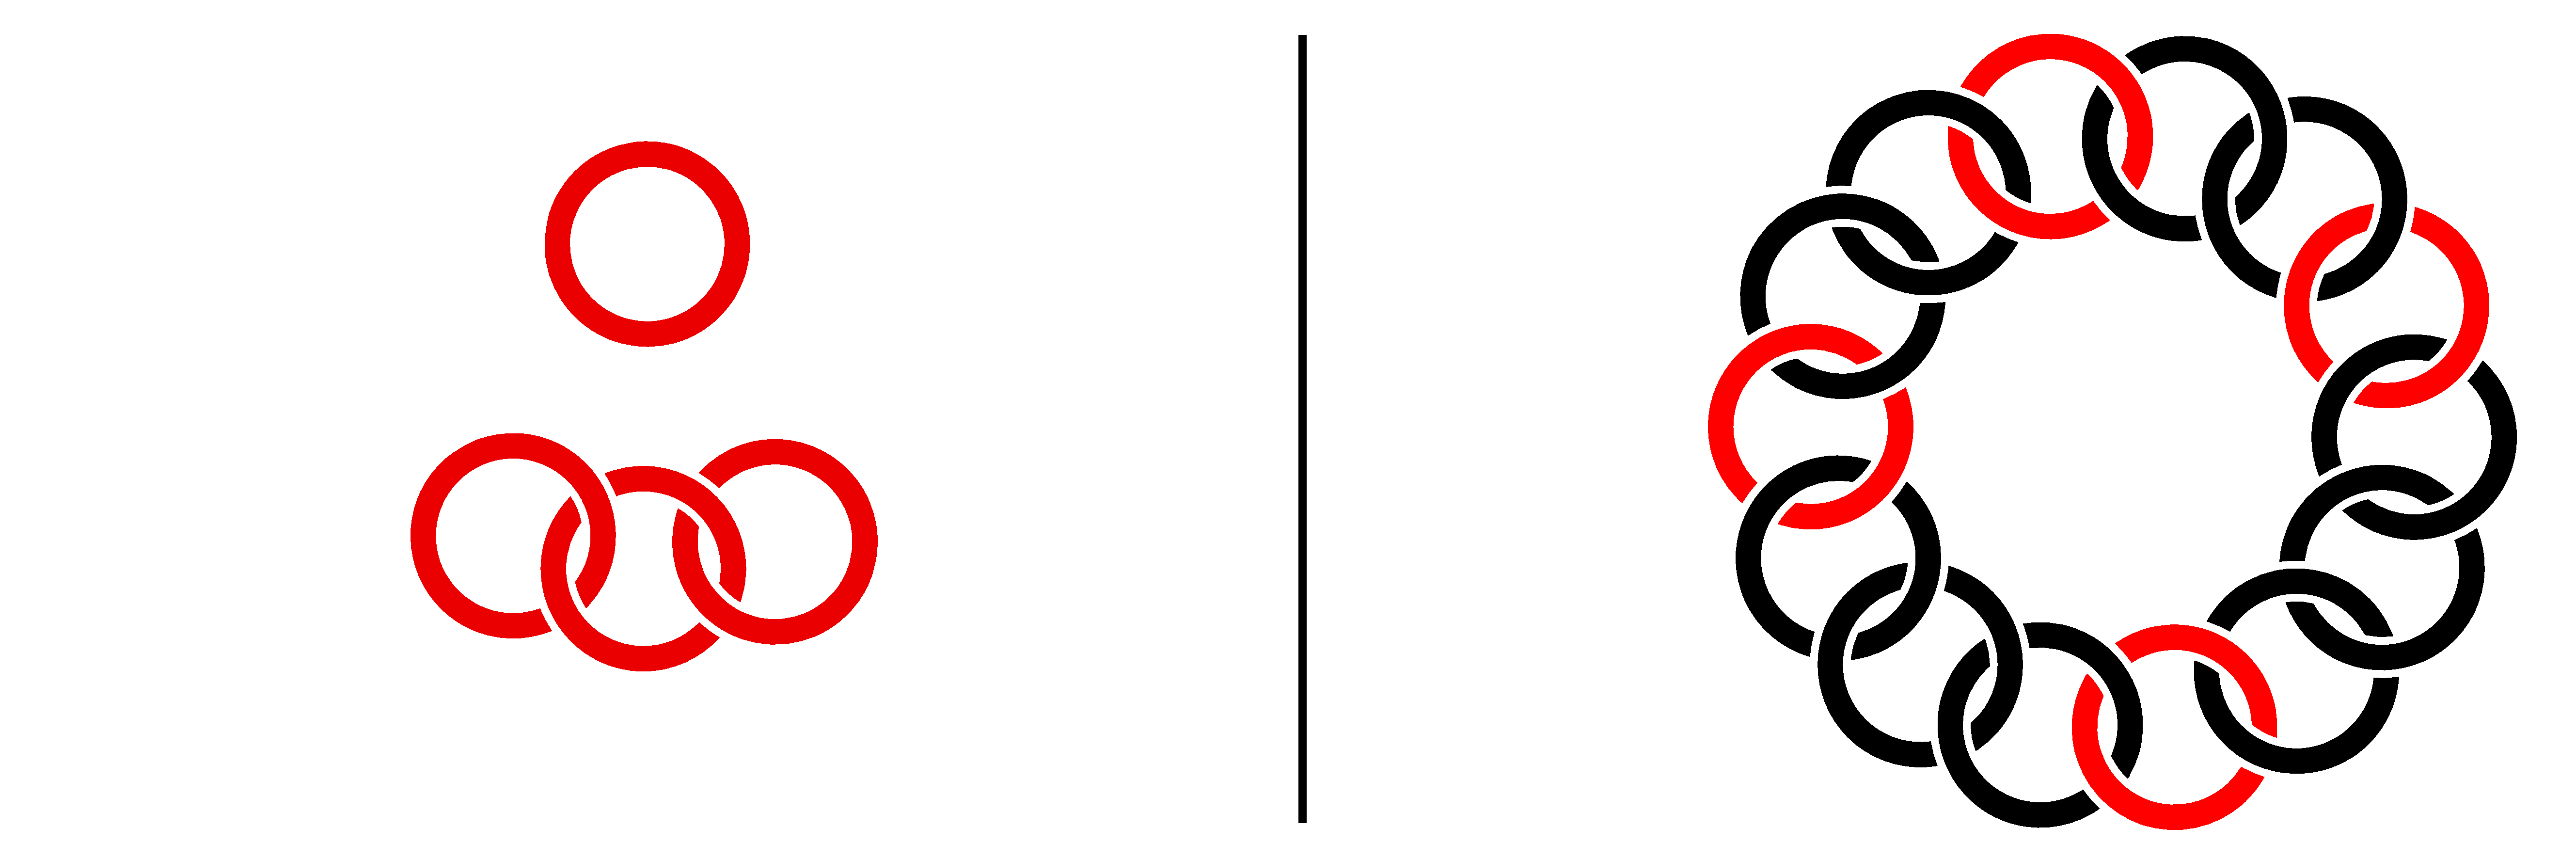
\includegraphics[width=0.75\linewidth]{example}
	\caption{In Test Case $2$ of Sample Input $1$, you can open up all chain links of the chains of length $1$ and $3$ to connect the remaining four chains.
		The resulting circular necklace can be seen on the right.}
\end{figure}

Unfortunately, this did not stop Eitri since he was gripped by pride when he got this task.
However, the smart dwarf noticed that the $n$ pieces were all simple chains, where the $i$th chain consists of $a_i$ interlocked chain links.
Thus, he could repair the chain by repeatedly opening a chain link, changing with which other chain links it was interlocked, and then closing the link again.
He knew that this was enough to make the chains form one circular necklace in the end, but he was not smart enough to figure out how to do this fast and get rid of the jinxed jewelry as soon as possible.
Suppose Eitri could open and close one chain link per minute, can you tell how long he would need?

\begin{Input}
	The input consists of:
	\begin{itemize}
		\item One line containing a single integer $t$, the number of test cases.
		\item $t$ descriptions of test cases, each consisting of:
			\begin{itemize}
				\item One line containing an integer $n$ $(1\leq n \leq 10^5)$, the
					number of chains.
				\item One line containing $n$ integers $a_1,\dots,a_n$ $(1\leq
					a_i < 10^5 \text{ for each $i$})$.
			\end{itemize}
		It is guaranteed that you have at least $3$ chain links in total.
	\end{itemize}
	It is guaranteed that the sum of $n$ over all test cases is at most $10^6$.
\end{Input}

\begin{Output}
	For each test case print the minimum time required to form a single circular necklace from the chains.
\end{Output}
